\section*{To Reviewer \#3}

\begin{shaded}
	\noindent\textbf{C1:} Some English mistakes.  If the authors have a native English speaking colleague, I would ask them for edits or run it by a professional editor.  I could follow the text, but there were some sentences that required me to stop and reread.  Again, nothing major, but it will help improve readability in a couple of places.
\end{shaded}
%
\noindent\textbf{Response:} 
We have carefully revised the manuscript and corrected the language issues as much as possible. We have also used the professional editing service Enago to improve the paper. 

\begin{shaded}
	\noindent\textbf{C2:} Some additional experiments would be nice.
	(a) Impact of table size on performance.  Does the proposed technique only work for specific table sizes?  It would be good to see a plot that varies the table size and shows how throughput changes across the different hash table implementations for the different datasets.
	(b) It would be nice to have a plot showing the memory use of the different hash table implementations relative to one another.  The number 4x is given but without much further explanation or detail.
\end{shaded}
%
\noindent\textbf{Response:} 
Our proposed approach works for tables with any size. 
In Figure 8, we demonstrate the performance by fixing the data size and varying the filled factor. 
A larger filled factor infers less memory is used.
Note that when fixing the data size and the filled factor at the same time, the memory sizes allocated for all GPU-based methods \underline{are almost identical}. 
Hence, we do not report the memory size of all compared methods.  
Due to space limit, we only present the result for the {\tt RAND} dataset.
We include the additional results for all datasets in this response (Figures 1-4 of the response), which share similar trends as those in the {\tt RAND} dataset.

\begin{minipage}{\textwidth}
	\begin{minipage}[b]{0.49\textwidth}\centering
		\begin{minipage}{0.49\textwidth}\centering
			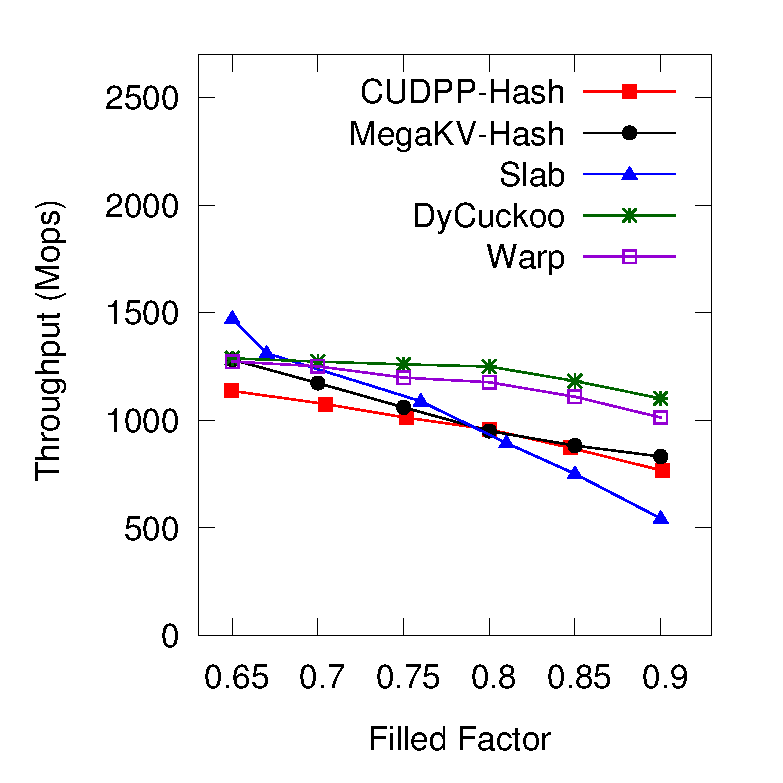
\includegraphics[width=\textwidth]{../pic/static-load_factor/ali/insert.eps}
			\centerline{\formal{insert}}
		\end{minipage}
		\begin{minipage}{0.49\textwidth}\centering
			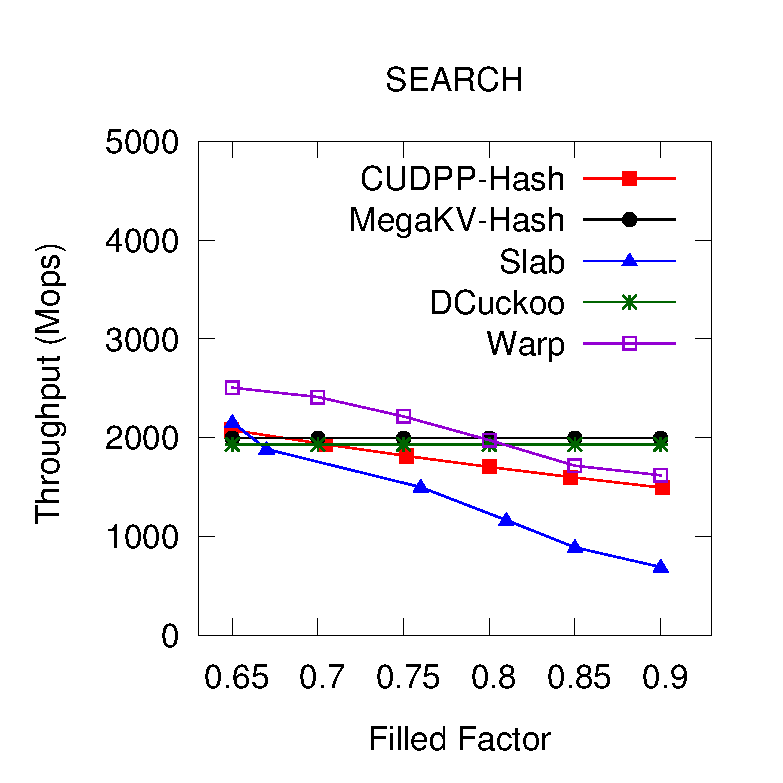
\includegraphics[width=\textwidth]{../pic/static-load_factor/ali/search.eps}
			\centerline{\formal{find}}
		\end{minipage}
	\captionof{figure}{Throughput of all compared approaches for varying the filled factor against the \dsali dataset.}
	\end{minipage}
	\hfill
	\begin{minipage}[b]{0.49\textwidth}
		\begin{minipage}{0.49\linewidth}\centering
			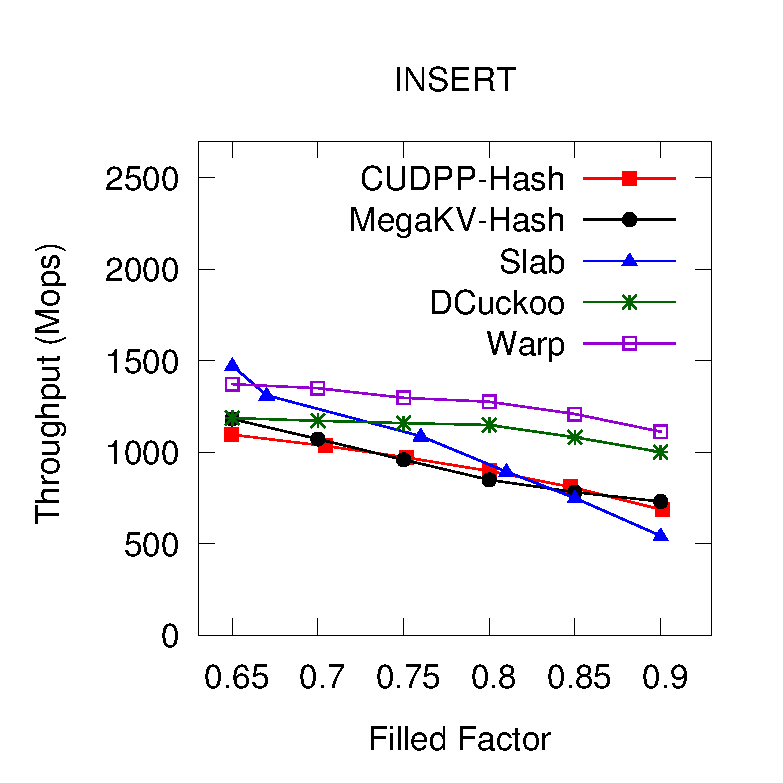
\includegraphics[width=\textwidth]{../pic/static-load_factor/reddit/insert.eps}
			\centerline{\formal{insert}}
		\end{minipage}
		\hfill
		\begin{minipage}{0.49\linewidth}\centering
			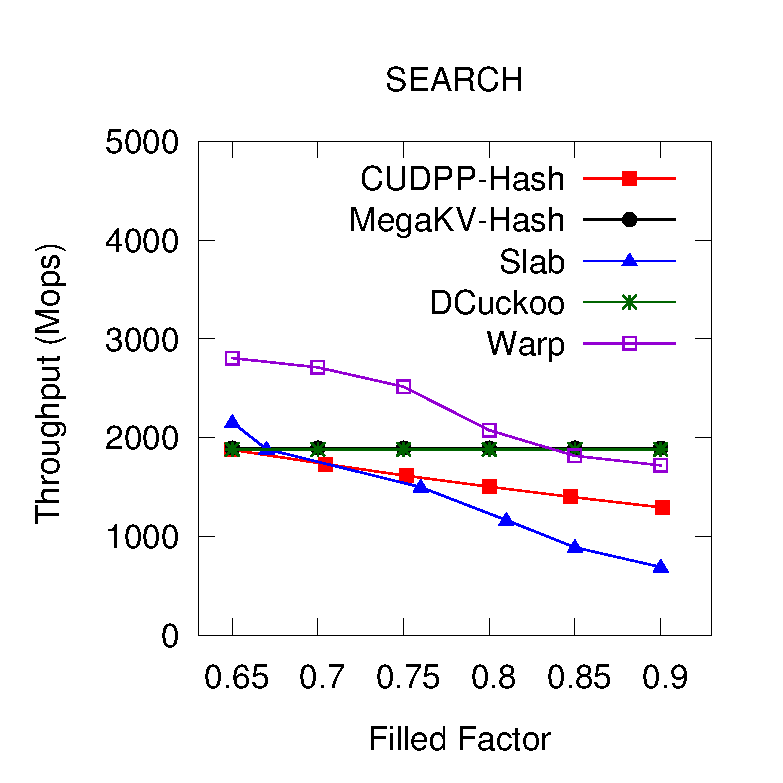
\includegraphics[width=\textwidth]{../pic/static-load_factor/reddit/search.eps}
			\centerline{\formal{find}}
		\end{minipage}
		\captionof{figure}{Throughput of all compared approaches for varying the filled factor against the \dsreddit dataset.}
	\end{minipage}
\end{minipage}

\begin{minipage}{\textwidth}
	\begin{minipage}[b]{0.49\textwidth}\centering
		\begin{minipage}{0.49\textwidth}\centering
			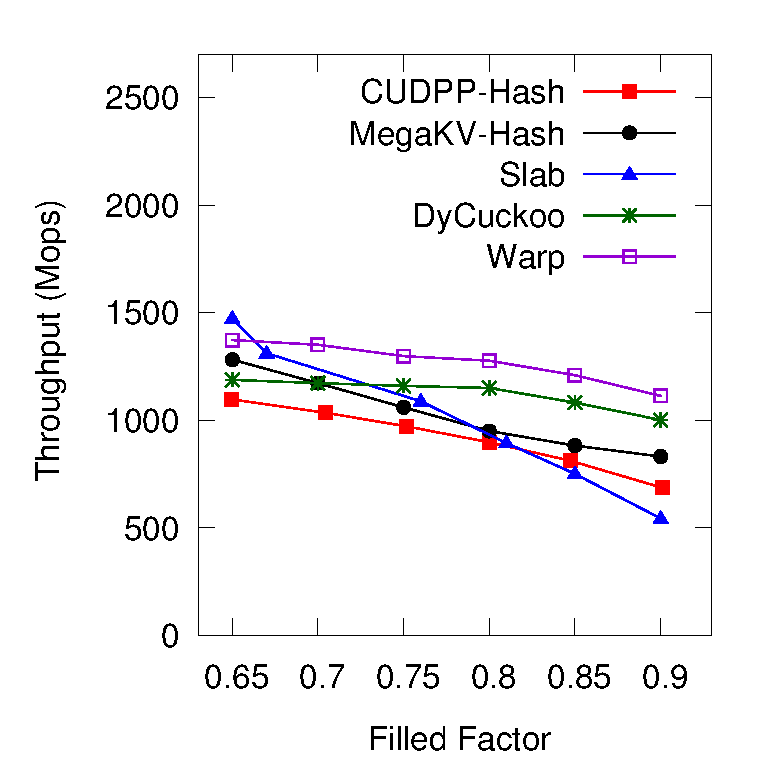
\includegraphics[width=\textwidth]{../pic/static-load_factor/twitter/insert.eps}
			\centerline{\formal{insert}}
		\end{minipage}
		\begin{minipage}{0.49\textwidth}\centering
			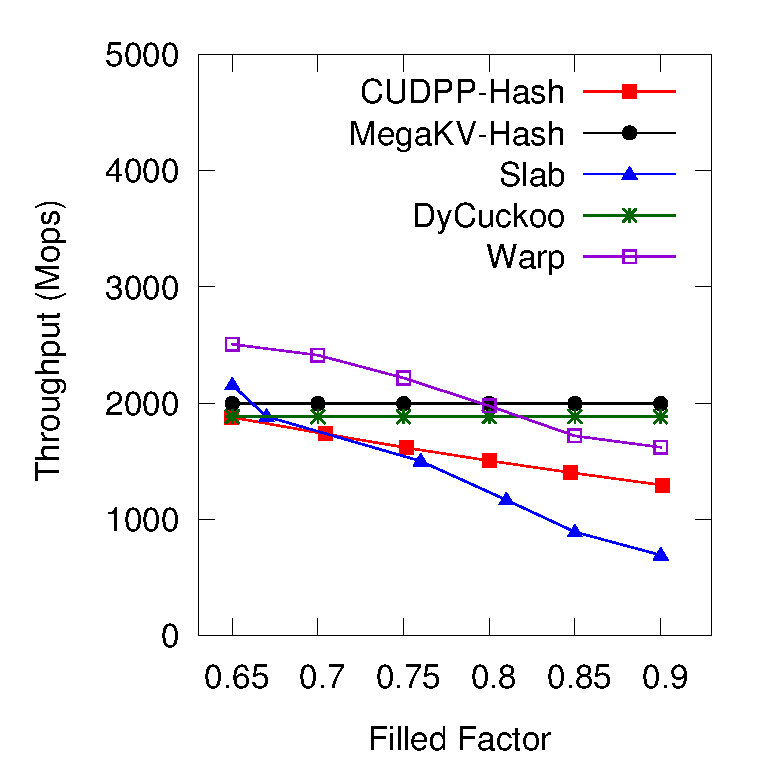
\includegraphics[width=\textwidth]{../pic/static-load_factor/twitter/search.eps}
			\centerline{\formal{find}}
		\end{minipage}
		\captionof{figure}{Throughput of all compared approaches for varying the filled factor against the \dstwitter dataset.}
	\end{minipage}
	\hfill
	\begin{minipage}[b]{0.49\textwidth}\centering
		\begin{minipage}{0.49\textwidth}\centering
			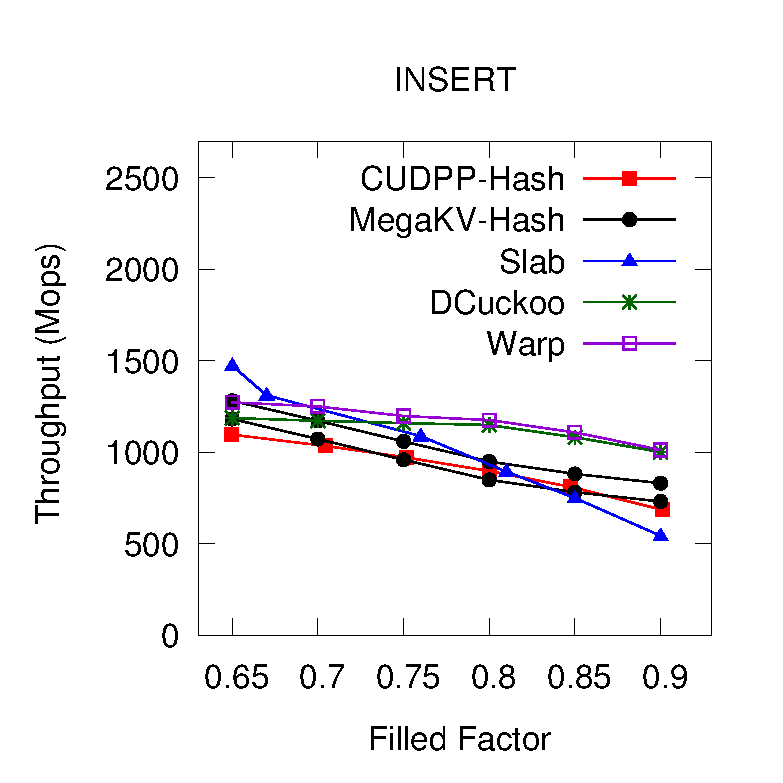
\includegraphics[width=\textwidth]{../pic/static-load_factor/tpch/insert.eps}
			\centerline{\formal{insert}}
		\end{minipage}
		\begin{minipage}{0.49\textwidth}\centering
			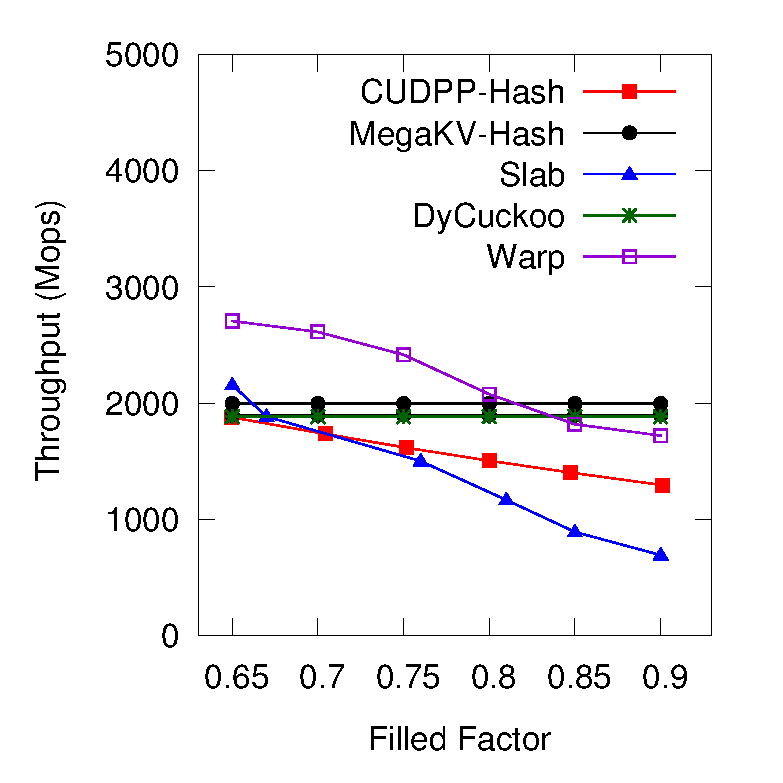
\includegraphics[width=\textwidth]{../pic/static-load_factor/tpch/search.eps}
			\centerline{\formal{find}}
		\end{minipage}
		\captionof{figure}{Throughput of all compared approaches for varying the filled factor against the \dstpch dataset.}
	\end{minipage}
\end{minipage}

\begin{shaded}
	\noindent\textbf{C3:} The proposed design applies updates at the granularity of batches.  While not inherently a problem, it means that fine-grain updates that have a required order need to be placed in different batches when using the current algorithms.
\end{shaded}
%
\noindent\textbf{Response:} 
We thank the reviewer for pointing out the issue. As GPUs are inherently built on a throughput-oriented architecture, small batches will lead to degraded performance. 
If the order of updates have to be enforced, CPUs are better choices for the scenario. 
We discuss the limitation of our approach in Section 6.4.

\begin{shaded}
	\noindent\textbf{C4:} Some missing citations.
	\begin{itemize}[noitemsep]
		\item The resizing approach shares similarities with the quotienting used in quotient filters see Bender et al. in VLDB'12 \cite{bender2012don}.  
		\item The hash-based partitioning with multiple hash tables is used in the radix-hash join \cite{boncz1999database} and in some high-performance group-and-aggregate algorithms.  
		\item The hierarchical approach also shares some similarities with recent work like the following although not exactly identical \cite{zuo2018write}
		\item See \cite{zhang2019data} for discussion on tradeoffs in data partitioning, a trait of this paper.
	\end{itemize} 	
\end{shaded}
%
\noindent\textbf{Response:} 
We thank the reviewer for pointing out these related works. We add these references as well as some discussions in this revision (Section~5.1). 

\begin{shaded}
	\noindent\textbf{C5:} 
	The references for the different datasets would be good for result reproducibility.
	Source code is not open-sourced.  I didn't see any mention of the source code being open-sourced.  Open sourcing the code would add to the potential impact of the work and aid in reproducibility.
\end{shaded}
%
\noindent\textbf{Response:} 
In the revised submission, we add the references for all datasets used in this paper except the {\tt COM} dataset due to confidentiality. We open-sourced our implementation and include the link in Section 6.